% % \part{数学建模实战}
% % \chapter{太阳影子定位}


% \documentclass[UTF8]{ctexbook}

% \ctexset{
%     part/number = \chinese{part}
% }

% \usepackage{multirow}
% \usepackage{amsmath}% ams 数学公式
% \usepackage{amsfonts}% ams 数学字体
% \usepackage{bbm}%重影字体
% \usepackage{amssymb,latexsym}% ams 数学符号与LaTeX数学符号
% \usepackage{mathrsfs}% 花式符号
% \usepackage{ntheorem}%定理、定义、证明
%     \theoremstyle{nonumberplain}
%     \theoremheaderfont{\bfseries}
%     \theorembodyfont{\normalfont}
%     \theoremsymbol{$\square$}
%     \newtheorem{Proof}{\hskip 2em 证明}
%     \newtheorem{theorem}{\hspace{2em}定理}[chapter]
%     \newtheorem{definition}{\hspace{2em}定义}[chapter] % 如果没有章, 只有节, 把上面的[chapter]改成[section]
%     \newtheorem{axiom}[definition]{\hspace{2em}公理}
%     \newtheorem{lemma}[definition]{\hspace{2em}引理}
%     \newtheorem{proposition}[definition]{\hspace{2em}命题}
%     \newtheorem{corollary}[definition]{\hspace{2em}推论}
%     \newtheorem{remark}{\hspace{2em}注}[chapter] %类似地定义其他“题头”. 这里“注”的编号与定义、定理等是分开的
%     \newtheorem{Assumption}{\hspace{2em}假设}[chapter]

% %算法伪代码
% %http://blog.csdn.net/lwb102063/article/details/53046265
% \usepackage{algorithm}
% \usepackage{algorithmicx}
% \usepackage{algpseudocode}
%     \floatname{algorithm}{算法}
%     \renewcommand{\algorithmicrequire}{\textbf{输入:}}
%     \renewcommand{\algorithmicensure}{\textbf{输出:}}
% % 罗马数字:示例:\rom{2}
% \makeatletter
% \newcommand*{\rom}[1]{\expandafter\@slowromancap\romannumeral #1@}
% \makeatother

% \usepackage{enumerate}%itemiz环境。\begin{enumerate}[step 1][a)]可以使用 A,a,I,i,1 作为可选项产生 \Alph,\alph,\Roman,\roman,\arabic 的效果
% \usepackage{cite}%参考文献
%     \bibliographystyle{plain}
% \usepackage{extarrows}% 带参数的箭头
% \usepackage{hyperref}% 超链接
% \usepackage{pifont}%然后在正文输入\ding{172}~\ding{211}得到相应数字,要是要①就输入:\ding{172}②就输:\ding{173}
% %\usepackage[CJKbookmarks, colorlinks, bookmarksnumbered=true,pdfstartview=FitH,linkcolor=black,citecolor=black]{hyperref}%超链接的格式设置
% \hypersetup{
%     colorlinks=false,% 去掉超链接颜色
%     pdfborder=0 0 0% 取消超链接的边框
% }
% \usepackage{graphicx}% 图片管理
% \usepackage{caption}
% \usepackage{subcaption}%并排的图各有标题
% \graphicspath{{images/}}% 设置图片搜索路径
% \usepackage{float,varwidth}% 浮动体
% \usepackage{booktabs}% 三线表
% \usepackage{fancyhdr}% 页眉设置
% \usepackage{xcolor}% 颜色宏包
% \usepackage{colortbl}% 彩色表格
% \usepackage{listings}% 代码高亮
% \usepackage{caption}% 对标题进行控制,如让\caption标题的字体缩小一号,同时数字标签使用粗体可以用:\usepackage[font=small,labelfont=bf]{caption}
% \usepackage{xfrac,upgreek}%分别是行间公式如a/b的形式(将原来的命令\frac改成\sfrac)和希腊字体的宏包的
% \usepackage{mathtools}%lgathered和rgathered环境把公式向左向右对齐
% \usepackage{tabularx}%提供自动延伸的表列,(X列格式说明符),文字过长时可以自动转行
% \usepackage{longtable}%长表格
% \usepackage{enumitem}%enumerate宏包的升级
% \usepackage{harpoon}%数学公式的矢量
% \usepackage{bookmark}%目录的书签
% \renewcommand{\headwidth}{\textwidth}%图片并排,这个要列在所有宏包的后面
% \definecolor{codegreen}{rgb}{0,0.6,0}
% \definecolor{codegray}{rgb}{0.5,0.5,0.5}
% \definecolor{codepurple}{rgb}{0.58,0,0.82}
% \definecolor{backcolour}{rgb}{0.95,0.95,0.92}
% \lstset{
%     commentstyle=\color{codegreen},
%     keywordstyle=\color{magenta},
%     numberstyle=\tiny\color{codegray},
%     stringstyle=\color{codepurple},
%     basicstyle=\footnotesize,
%     breakatwhitespace=false,% 断行只在空格处
%     breaklines=true,% 自动断行
%     captionpos=b,% 标题位置
%     keepspaces=true,
%     numbers=left,
%     numbersep=5pt,
%     showspaces=false,
%     showstringspaces=false,
%     showtabs=false,% 显示
%     tabsize=2% TAB 被当作两个空格
% }
% \topmargin=0pt\oddsidemargin=0pt\evensidemargin=0pt
% \textwidth=16.5cm\textheight=23cm\raggedbottom%我这么设置是为了缩小页边距,满足有的文字无法转行
% \pagestyle{headings}%页眉为章节标题,无页脚
% \setlength{\abovecaptionskip}{10pt}
% \setlength{\belowcaptionskip}{-15pt}%图片表格的前后距离设置
% \CTEXsetup[format={\zihao{-3}\raggedright\bfseries}]{section}%设置节的格式
% \begin{document}
% \part{数学建模实战}
\chapter{太阳影子定位}
\section{题目要求}
    \par
    \textbf{A题:太阳影子定位}
    \par
    如何确定视频的拍摄地点和拍摄日期是视频数据分析的重要方面,太阳影子定位技术就是通过分析视频中物体的太阳影子变化,确定视频拍摄的地点和日期的一种方法。
    \par
    1.建立影子长度变化的数学模型,分析影子长度关于各个参数的变化规律,并应用你们建立的模型画出2015年10月22日北京时间9:00-15:00之间天安门广场(北纬39度54分26秒,东经116度23分29秒)3米高的直杆的太阳影子长度的变化曲线。
    \par
    2.根据某固定直杆在水平地面上的太阳影子顶点坐标数据,建立数学模型确定直杆所处的地点。将你们的模型应用于附件1的影子顶点坐标数据,给出若干个可能的地点。
    \par
    3. 根据某固定直杆在水平地面上的太阳影子顶点坐标数据,建立数学模型确定直杆所处的地点和日期。将你们的模型分别应用于附件2和附件3的影子顶点坐标数据,给出若干个可能的地点与日期。
    \par
    4.附件4为一根直杆在太阳下的影子变化的视频,并且已通过某种方式估计出直杆的高度为2米。请建立确定视频拍摄地点的数学模型,并应用你们的模型给出若干个可能的拍摄地点。
    \par
    如果拍摄日期未知,你能否根据视频确定出拍摄地点与日期?
    \subsection{附件1}
        \par
        说明:坐标系以直杆底端为原点,水平地面为$xy$平面。直杆垂直于地面。测量日期:2015年4月18日。附件1数据如表(\ref{太阳影子定位:附件1})所示
        \begin{table}[H]
        \caption{太阳影子定位:附件1}
        \label{太阳影子定位:附件1}
        \centering
        \begin{tabular}{cc||cc}
        \toprule
        $t_i$(北京时间) & $l_i$影长(米) & $t_i$(北京时间) & $l_i$影长(米) \\
        \midrule
        14:42 &   1.1496 &  15:15 &  1.5402\\
        14:45 &   1.1822 &  15:18 &  1.5799\\
        14:48 &   1.2153 &  15:21 &  1.6201\\
        14:51 &   1.2491 &  15:24 &  1.6613\\
        14:54 &   1.2832 &  15:27 &  1.7033\\
        14:57 &   1.3180 &  15:30 &  1.7462\\
        15:00 &   1.3534 &  15:33 &  1.7901\\
        15:03 &   1.3894 &  15:36 &  1.8350\\
        15:06 &   1.4262 &  15:39 &  1.8809\\
        15:09 &   1.4634 &  15:42 &  1.9279\\
        15:12 &   1.5015 &    {}  &{} \\
        \bottomrule
        \end{tabular}
      \end{table}

\section{太阳影子定位研究}
    \subsection{模型的假设}
        \begin{enumerate}
        \item 假设研究的物体是垂直于该地点的切平面;
        \item 影子长度仅考虑切平面上的投影长,不考虑弧度;
        \item 假设地球为球体;
        \item 假设一天时间内,太阳直射点的纬度不变(赤纬角在一天内保持不变);
        \item 不同年份的同一时间、同一地点的太阳高度角是相同的;
        \item 假设地球绕太阳公转的轨道为圆形轨道。
        \end{enumerate}
    \subsection{符号说明}

    \subsection{问题一的分析与求解}
        \subsubsection{问题的分析}
            \par
            建立影子长度变化的数学模型,分析影子长度关于各个参数的变化规律,并应用你们建立的模型画出2015年10月22日北京时间9:00-15:00之间天安门广场(北纬39度54分26秒,东经116度23分29秒)3米高的直杆的太阳影子长度的变化曲线。
            \par
            第一问的主要目标是让我们确定要分析的量,并建立各个量之间的函数关系。
        \subsubsection{模型的建立与求解}
            \par
            我们要通过物体影子的数据(各时刻的长度变化和方向变化)来判定物体的位置(经纬度)及拍照时间。
            某固定杆高的影子长度在不同地点和时点下应该是不同的。可以推测影长是关于杆高、日期、时间、经度和纬度的函数,事实也确实如此。下面,我们找出各变量间具体的函数关系。在建立函数关系式之前,我们对太阳直射点、赤纬角和时角等相关概念做了了解,并给出了某日某时杆高为$h$的观测物在地球某点$O$处的太阳影长变化图,如图(\ref{fig:太阳影子长度模拟图})所示
			\begin{figure}[H]
			\centering
			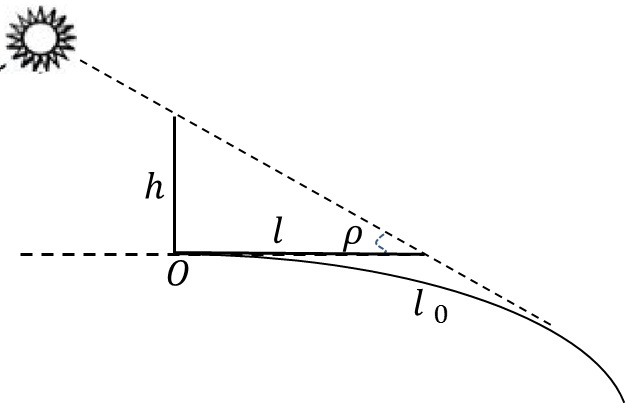
\includegraphics[height=4cm]{images/Sun_shadow_length_simulation.jpg}
			\caption{太阳影子长度模拟图}
			\label{fig:太阳影子长度模拟图}
			\end{figure}
            \par
            假设研究的物体是垂直于该地点的切平面;并且影子长度仅考虑切平面上的影长,不考虑弧度。由于地球半径很大,杆子在地球表面的影长$l_0$可以用杆子所在切平面上的影长$l$做近似代替,由此可建立杆高$h$(观测物的高度)关于影长$l$(真实影长$l_0$的估计值)和太阳高度角$\rho$的关系式
            \begin{align*}
            % h = l \tan\rho = \frac{l\sin\rho}{\sqrt{1-\sin^2\rho}}\\
            l = \frac{h}{\tan\rho} = \frac{h\sqrt{1-\sin^2\rho}}{\sin\rho}
            \end{align*}
            其中:$\rho$是太阳光线与拍摄地点切平面的交角,称为太阳高度角。我们设经度为$\theta$,纬度为$\varphi$,年份为$y$,日期为$n$,时刻为$t$,杆高为$h$,影长为$l$。应该可以想到的是$\rho$是$\varphi,\theta,n,t,y$的函数,那么,这种函数关系到底是怎样的呢?为简单处理,假设不考虑$y$对$\rho$的影响,即不同年份的同一时间、同一地点的太阳高度角是相同的。下面,我们来求解$\rho$或者$\sin\rho$。
            \par
            假设地球是一球体,以其球心为坐标原点,以赤道面作为$xoy$面,以垂直$xoy$向北的方向为$z$轴方向建立三维直角坐标系$oxyz$,如图(\ref{fig:地球坐标系})所示
			\begin{figure}[H]
			\centering
			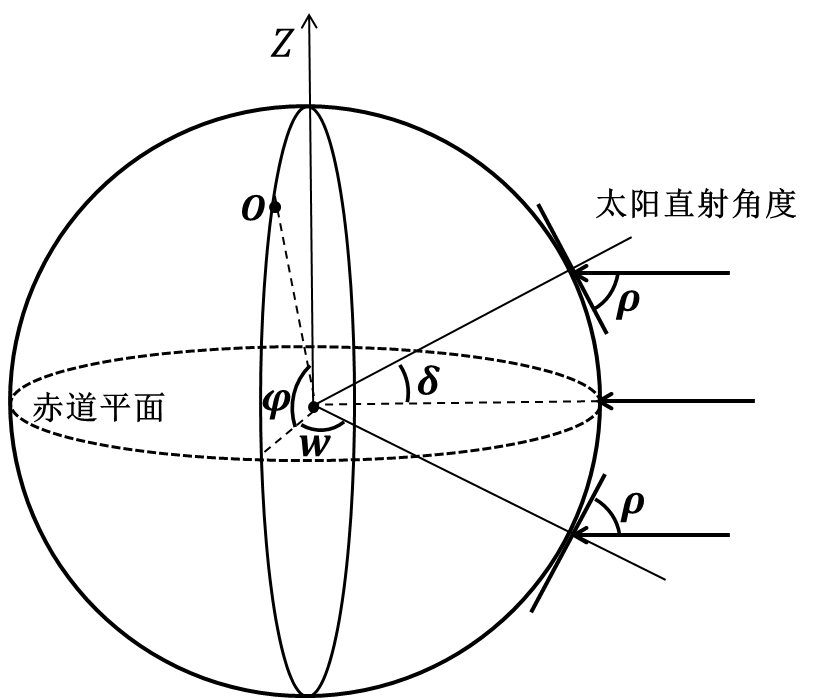
\includegraphics[height=4cm]{images/Earth_coordinate_system.jpg}
			\caption{地球坐标系}
			\label{fig:地球坐标系}
			\end{figure}
            图中$w$为太阳时角,$\delta$为太阳直射点维度(太阳赤纬),$O$为待求地点,$\varphi$为$O$点的纬度。我们假设一天内太阳直射点的维度不变,在给出$\rho$之前,有一些常识要说明
            \begin{enumerate}
            \item 太阳直射点的太阳高度角为$90^\circ$;
            \item 太阳赤纬是太阳直射点的纬度$\delta$,其一年内的变化情况如图(\ref{fig:太阳赤纬一年的变化情况})示意图
			\begin{figure}[H]
			\centering
			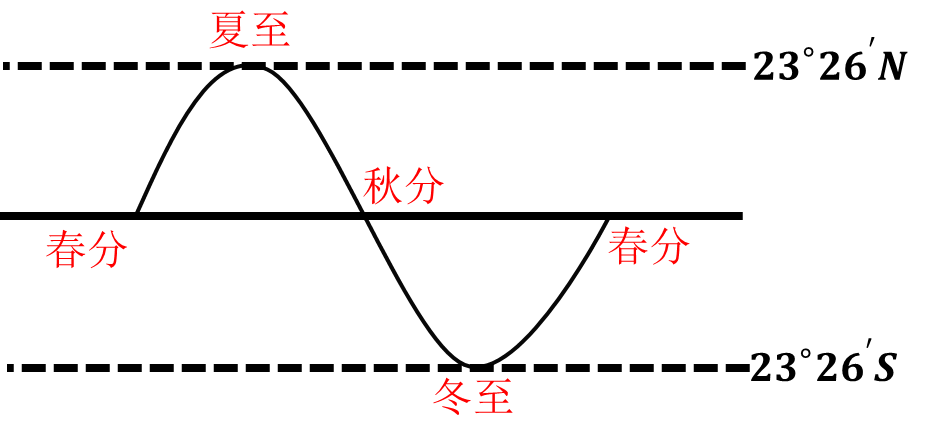
\includegraphics[height=4cm]{images/Changes_in_the_sun_declination.jpg}
			\caption{太阳赤纬一年的变化情况}
			\label{fig:太阳赤纬一年的变化情况}
			\end{figure}
            \item 太阳光线到达地球时时平行的(这点需要假设);
            \item 以太阳直射点为圆心的圆上各地点的太阳高度角近似相等;
            \item 自转改变太阳直射点的经度,公转改变维度。
            \end{enumerate}
            \par
            我们知道,太阳高度角$\rho$是线(太阳光线)与面(待求地点$O$的切平面)的夹角,因此,我们需要知道平面的法向量以及线的向量。$O$点所在的切平面的单位法向量为
            \begin{align*}
            \vec{n} = (\cos\varphi\cos w,\cos\varphi\sin w,\sin\varphi)
            \end{align*}
            而第$n$天$t$时刻的入射向量为
            \begin{align*}
            \vec{m} = (-\cos\delta,0,-\sin\delta)
            \end{align*}
            则$O$点的太阳高度角$\rho$(如图(\ref{fig:太阳照射点的投影向量})所示)求解为
            \begin{align*}
            \sin\rho = -\vec{n}\cdot\vec{m} = \cos\varphi\cos\delta\cos w+\sin\varphi\sin\delta
            \end{align*}
            其中:$\delta$为太阳赤纬,$w$为太阳时角。
			\begin{figure}[H]
			\centering
			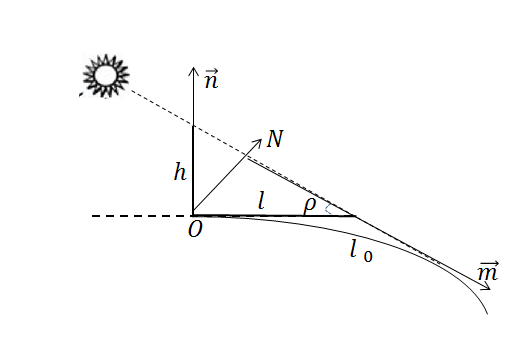
\includegraphics[height=4cm]{images/Projection_Vector_of_Solar_Irradiation_Point.jpg}
			\caption{太阳照射点的投影向量}
			\label{fig:太阳照射点的投影向量}
			\end{figure}
            \par
            关于赤纬角$\delta$的计算方法有:Cooper 法、Spencer 法、Stome法、Bpirges 法等;而关于太阳时角$w$的计算方法亦有:Wloof 法、Spencer 法、Whillier 法、Lamm法等。杜春旭等人在《 一种高精度太阳位置算法》 一文中对上述算法进行了分类比较,显示在每天世界$0$时时,Bpirges 法和Lamm法求解的$\delta$和$w$的误差较小,结果较为精确。现在我们引用Spencer在1971年给出的赤纬角$\delta$(弧度)的计算公式
            \begin{align*}
            \delta &= 0.006918 - 0.399912 \cos(\Gamma) + 0.070257 \sin(\Gamma) - 0.006758 \cos(2\Gamma)\\
            &\quad + 0.00907 \sin(2\Gamma) - 0.002697\cos(3\Gamma) + 0.00148\sin(3\Gamma)
            \end{align*}
            其中:$\Gamma = 2\pi(n- 1)/365$,单位为弧度,$n$ 表示一年中的第$n$天即日期,如1 月 1 日计$ n=1 $,12 月 31 日的计$n=365$。
            \par
            \textbf{太阳赤纬角:}下面,我们尝试给出太阳赤纬$\delta$的求解。设地球$P$绕太阳$S$公转的轨道为圆形轨道。太阳位于圆形轨道的圆心,以太阳为原点,以圆形轨道面(黄道平面)为$xoy$面家里公转坐标系,如图(\ref{fig:公转坐标系})所示
			\begin{figure}[H]
			\centering
			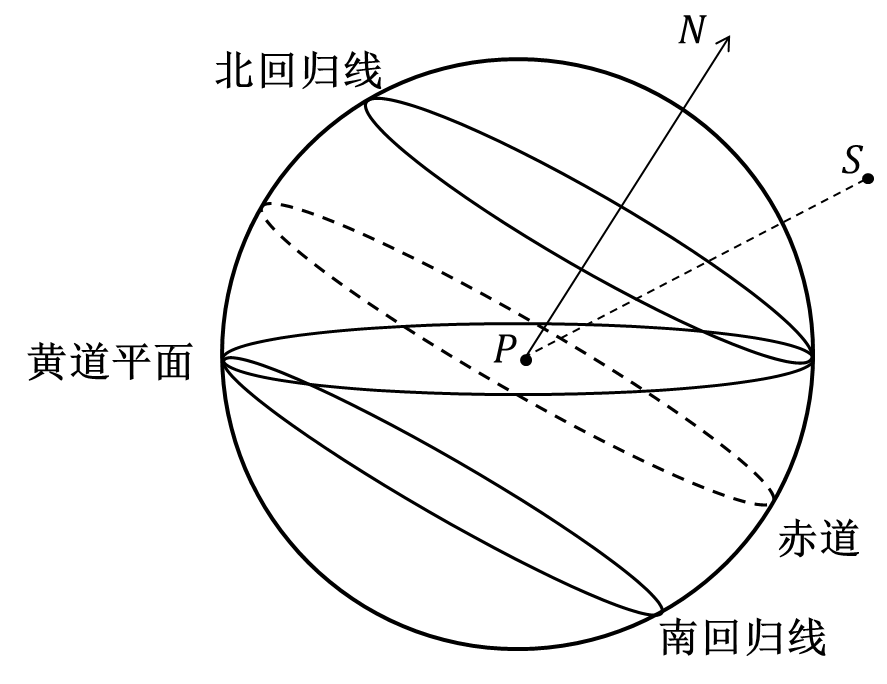
\includegraphics[height=4cm]{images/Revolving_coordinate_system.jpg}
			\caption{公转坐标系}
			\label{fig:公转坐标系}
			\end{figure}
            设一年有$T^*$天,一天有$t^*$小时,以春分(3月21日)为第0天($n=0$),则第$n$天$t$时刻,地球的坐标为
            \begin{align*}
            P(r\cos\frac{2\pi T}{T^*},r\sin \frac{2\pi T}{T^*},0)
            \end{align*}
            其中:$r$为地球中心到太阳中心的距离,$T = n+\frac{t}{t^*}$。
            \par
            设第$n$天$t$时刻,太阳直射地球的维度$\delta$(太阳赤纬),已知在春分$t_0$时刻太阳直射赤道,即当$n=0,t=t_0$时,$\delta=0$,此时的$T$为$T_0\frac{t_0}{t^*}$。而地球中心坐标为
            \begin{align*}
            P_0(r\cos\frac{2\pi T_0}{T^*},r\sin \frac{2\pi T_0}{T^*},0)
            \end{align*}
            设北回归线的纬度为$\delta_0$,则北极方向是$(0,0,1)$绕$SP_0$轴旋转$\delta_0$后的方向。在地球绕太阳公转过程中,北极方向始终保持不变,因而
            \begin{align*}
            \overrightarrow{PN} = \left( \sin \frac{2\pi T_0}{T^*}\sin\delta_0,-\cos\frac{2\pi T_0}{T^*}\sin\delta_0,\cos\delta_0 \right)
            \end{align*}
            $\overrightarrow{PS}$与$\overrightarrow{PN}$的夹角为$\frac{\pi}{2}-\delta$,因此
            \begin{align*}
            \cos(\frac{\pi}{2}-\delta) = \frac{\overrightarrow{PS}\cdot\overrightarrow {PN}}{|\overrightarrow{PS}||\overrightarrow {PN}|}
            \end{align*}
            即
            \begin{align*}
            \sin\delta = -\cos\frac{2\pi T}{T^*}\sin\frac{2\pi T_0}{T^*}\sin\delta_0+\sin\frac{2\pi T}{T^*}\cos\frac{2\pi T_0}{T^*}\sin\delta_0 = \sin\frac{2\pi \left( n+\frac{t-t_0}{t^*} \right) }{T^*}\sin\delta_0
            \end{align*}
            为简单,假设赤纬角在一天内保持不变,则上式可写为
            \begin{align*}
            \sin\delta=\sin\frac{2\pi n}{T^*}\sin\delta_0
            \end{align*}
            \par
            \textbf{太阳时角:}定义太阳时角$w$在正午时为$0^\circ$,每隔一小时增加$15^\circ$,上午为正,下午为负。但考虑到实际两地之间存在时差并对时角产生影响,且中国各地区均以北京时间为标准(北京位于$120^\circ E$,所在时区为东 8 区)因此某地以北京时间为依据的时角$w$(弧度化)的计算公式为
            \begin{align*}
            w = \frac{\pi (12-t)15^\circ}{180^\circ}+\frac{\pi}{180^\circ}\left\{
            \begin{aligned}
            & 120^\circ-\theta \quad \theta\in [0,180^\circ E]\\
            & 120^\circ+\theta \quad \theta\in [0,60^\circ W]\\
            & 240^\circ-\theta \quad \theta\in [60,180^\circ W]
            \end{aligned}
            \right.
            \end{align*}
            其中:$w$为时角,$t$为时间(以小时为单位,可为小数,如13.326),$θ$为经度。
            \par
            通过以太阳高度角 赤纬角$\delta$和太阳时角$w$为桥梁,搭建了影长$l$关于杆高$h$、日期$n$、时间$t$、经度$\theta$和纬度$\varphi$的具体函数关系式。依据此关系式,可以解决下列关于太阳影子定位的问题:
            \begin{enumerate}
            \item 给出具体的$\varphi$、$\theta$、$n$、$h$,观察$l$随$t$的变化;
            \item 给出具体的$n$、$h$、$t$,观察$l$随$\varphi$、$\theta$的变化;
            \item 给出一组$(t_i,l_i )   i=1,2,\dots,k$,($k$ 为观测个数,$t_i,l_i$皆可在具体的视频中求得),在$n$已知$h$未知但固定的条件下,求出视频的拍摄位置$\varphi,\theta$;
            \item 给出一组$(t_i,l_i )   i=1,2,\dots,k$, $h$未知但固定的条件下,求出视频的拍摄位置$\varphi,\theta$和拍摄日期$n$;
            \end{enumerate}
            \par
            针对问题1和问题2,可通过各参数间的函数关系式绘制图像进行分析,相对简单。问题4在问题3的基础上增加了一个参数n的求解,因此,我们将详细讨论问题3的求解,简要分析问题4。
            对模型求解之前,我们做如下规定:由于问题中的参数很多,均以如下表达式规范参数
            \begin{align*}
            y = f(x;\alpha,\beta|C)
            \end{align*}
            其中:$y$表示输出变量(可以是标量也可以是向量),$x$表示出入变量(可以是标量也可以是向量),$\alpha,\beta$表示参数,$C$表示某变量的固定值。
        \subsubsection{程序}
            \par
            Matlab给出了一个求解影长变化的示例\footnote{http://cn.mathworks.com/help/matlab/examples/live-editor-intteractive-narrative.html},可以作为参考。下面,我们给出3m长杆9点到15点太阳影子长度变化求解程序,其中Rad2deg函数是将角度转化为弧度,numdate函数是用于计算天数$n$,求解程序如下:
            \begin{lstlisting}[language = Matlab]
            phi = Rad2deg(39,54,26);%纬度(角度转化为弧度)
            theta = Rad2deg(116,23,29);%经度
            h = 3;%杆高
            n = numdate(2015,10,22);%天数n
            t = [9:0.2:15];
            for i = 1:length(t)
                Gamma = 2*pi*(n-1)/365;%弧度
                delta = 0.006918-0.399912*cos(Gamma)+0.070257*sin(Gamma)...
                    -0.006758*cos(2*Gamma)+0.000907*sin(2*Gamma)-0.002697*cos(3*Gamma)+0.00148*sin(3*Gamma);%弧度
                w = (12-t(i))*15*pi/180+Rad2deg(3,36,31); %弧度
                sin_rho = sin(phi)*sin(delta)+cos(phi)*cos(w)*cos(delta);
                l(i) = h*sqrt(1-sin_rho^2)/sin_rho;
            end
            figure
            plot(t,l,'r-')
            set(gca,'XTick',[9:15])
            set(gca,'XTickLabel',{'9:00','10:00','11:00', '12:00','13:00','14:00','15:00'})
            xlabel('北京时间')
            ylabel('杆影子长/m')
            title('3m长杆9点到15点太阳影子长度变化曲线图')
            \end{lstlisting}
        \subsubsection{结果}
            \par
            3m长杆9点到15点太阳影子长度变化曲线图如图(\ref{fig:3m长杆9点到15点太阳影子长度变化曲线图(无插值)})所示
			\begin{figure}[H]
			\centering
			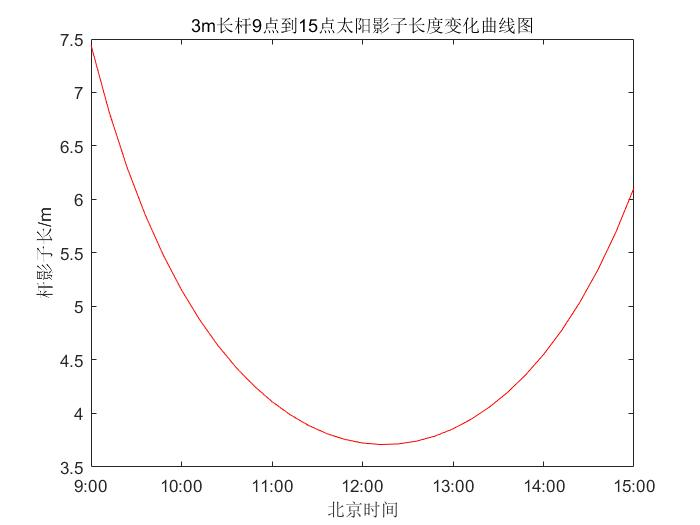
\includegraphics[width = 8cm]{images/3m_pole_sun_shadow_length_change1.jpg}
			\caption{3m长杆9点到15点太阳影子长度变化曲线图(无插值)}
			\label{fig:3m长杆9点到15点太阳影子长度变化曲线图(无插值)}
			\end{figure}

    \subsection{问题二的分析与求解}
        \subsubsection{问题的分析}
            \par
            根据某固定直杆在水平地面上的太阳影子顶点坐标数据,建立数学模型确定直杆所处的地点。将你们的模型应用于附件1的影子顶点坐标数据,给出\underline{若干个可能}的地点。
            \par
            通过抓帧工具获得某一视频中的$(t_i,l_i ) $ 数据$k$组$(i=1,2,\dots,k)$,且视频的拍摄日期$n$已知,杆高$h$固定(可分为已知和未知),利用$k$组$(t_i,l_i )$数据求解视频的拍摄位置$(\varphi,\theta)$。针对此问题,基本思想是利用最小二乘法求解$l=f(t;\varphi,\theta|n,h)$中的参数$(\varphi,\theta)$,并给定输入变量$t$和输出变量$l$的$k$组观测值$(t_i,l_i )(i=1,2,\dots,k)$进行求解,使总离差平方和最小的$(\varphi,\theta)$即为所求。然而这种方法并不适用于杆高$h$未知的情况,即使转化为$h=f(t,l;\varphi,\theta|n)$仍无法求解,因此需重新考虑。既然各变量关系已知,给出了$k$组$(t_i,l_i )$的观测值,那么每代入一组$(t_i,l_i )$都会有一个杆高$h$的估计值$h_i$,相应的会得到$k$组$h_i$,由于真实杆高$h$未知但固定,可详细分析。

        \subsubsection{模型的建立与求解}
            \par
            \textbf{方法1:最小二乘模型}
            \par
            根据附件1中的点坐标$(x_i,y_i)$我们可以求出杆的影长$\hat{l}_i(i=1,2,\dots,k)$。当然,我们还可以根据影长公式
            \begin{align}
            \label{太阳影子:影长公式}
            l_i = \frac{h}{\sqrt{\tan \rho_i}}
            \end{align}
            我们可以求解$(\varphi,\theta)$使真实值$l_i$与测量值$\hat{l}_i$的离差平方和最小(最小二乘),即
            \begin{align*}
            \min_{\varphi,\theta}\  J(\varphi,\theta) = \sum_{i=1}^k (l_i-\hat{l}_i)^2
            \end{align*}
            \par
            但是,上面计算影长的公式(\ref{太阳影子:影长公式})的杆高$h$未知,这使得问题变得困难。其实,这里我们可以任意设置一个杆高$h$(只要有就可以了),在计算的过程中杆高的影响会消失,我们仍能求解出最佳的地点$(\varphi,\theta)^*$。
            \par
            \textbf{方法2:比例模型}
            \par
            上面的分析中杆高$h$未知,我们可以想办法消去杆高$h$。将各影长相除,我们研究影长变化的改变。考虑相邻两个影长的变化,有
            \begin{align*}
            \min_{\varphi,\theta}\ J(\varphi,\theta) = \sum_{i=1}^{k-1} \left( \frac{l_{i+1}}{l_i} - \frac{\hat{l}_{i+1}}{\hat{l}_i} \right) ^2
            \end{align*}
            上面的模型中不再要求$h$已知。其实,我们还可以建立更一般的目标
            \begin{align*}
            \min_{\varphi,\theta}\ J(\varphi,\theta) = \sum_{j=i+1}^k\sum_{i=1}^{k-1} \left( \frac{l_{j}}{l_i} - \frac{\hat{l}_{j}}{\hat{l}_i} \right) ^2
            \end{align*}
            \par
            \textbf{方法3:最小方差模型}
            \par
            最小方差模型是基于下面的思想:真正的视频拍摄位置$(\varphi,\theta)$会使得$\forall i,j\in [1,k]$有$h_i=h_j$成立,即杆高$h$的估计值$h_i$每次求解都相等$h_1=h_2=\cdots=h_k$。越接近真实的$(\varphi,\theta)$估计值$h_i,h_j$之间的偏差越小,即
            \begin{align*}
            \min_{\varphi,\theta}\ J(\varphi,\theta) = \sum_{i,j}|h_i-h_j|
            \end{align*}
            \par
            但上面目标处理起来并不是很方便,我们将其转化为下面的优化问题
            \begin{align*}
            \min_{\varphi,\theta}\ \left\{
            \begin{aligned}
            & \frac{1}{k}\sum_{i=1}^k(h_i - \mathbb{E}(h_i))^2 = \mathrm{Var}(h_i)\quad&  \text{unknown }h\\
            & \frac{1}{k}\sum_{i=1}^k(h_i-h)^2 \quad&  \text{known }h
            \end{aligned}
            \right.
            \end{align*}
            其中:$h$表示已知的杆高,$h_i$为杆高的估计值,$\mathbb{E}(h_i)$为杆高的估计值的期望,$Var(h_i)$为杆高的估计值的方差,$k$为观测组数。
            \par
            要对上述优化模型进行求解,提出的简单直观的想法是:遍历地球上所有的地点$(\varphi,\theta)$,每个$(\varphi,\theta)$都会有$h_i$,找到$\min Var(h_i )$所在的$(\varphi,\theta)^*$即可。这种做法的求解结果虽然精确,但计算量却异常大;且因为需要遍历更多的点所以精度越高计算量越大。
            基于这种思想,且考虑到计算的精度和时间,设计了粗劣搜索算法+精确搜索算法对问题进行求解。
            \par
            上面建立了3个不同的优化模型,下面我们来考虑相应的约束条件。首先,纬度应该在$\pm 90^\circ$之间,即$-90^\circ<\varphi<90^\circ$;此外,直杆的影子只有在存在太阳直射的地方才能出现,所以要约束$\rho>0$。由此有最终的优化模型
            \begin{align*}
            & \min_{\varphi,\theta}\ J(\varphi,\theta)\\
            & s.t.\left\{
            \begin{aligned}
            & -90^\circ<\varphi<90^\circ\\
            & \rho_i>0\\
            & i=1,2,\dots,k
            \end{aligned}
            \right.
            \end{align*}

        \subsubsection{程序}
            \par
            根据影子长度的变化,还可以判断出当地时间是上午还是下午,影子长度单调递增是下午。对于上述的3个优化模型,可以使用牛顿法、拟牛顿法或者遗传算法等进行求解。还可以采用搜索算法进行求解,搜索法本质上是枚举,将优化变量按一定精度离散化,得到一系列离散值,对所有这些离散值进行枚举,寻找其中的最优解及最优值。搜索算法编程较为容易,但工作量大,为了减少搜索时间,可以采用变步长搜索法,即先用较大的精度对优化变量离散,搜索得到其中的最优解,然后缩小精度,在最优解附近按更小精度离散化后再进行搜索。
            \par
            问题二的求解程序如下,这里我们仅给出模型一:最小方差模型的求解程序
            \begin{lstlisting}[language = Matlab]
            %%%%%%%%%%%%%%%%%%%%%%%%%%%%%模型一:最小方差模型%%%%%%%%%%%%%%%%%%%%%%%%%%%%%
            clc,clear
            %部分量输入
            n = numdate(2015,4,18);%日期
            for i=1:6
                t(i)=time2h(14,42+3*(i-1));
            end
            for i=7:21
                t(i)=time2h(15,0+3*(i-7));
            end
            l = [1.149625826 1.182198976 1.215296955 1.249051052 1.28319534 1.317993149 ...
            1.353364049 1.389387091 1.426152856 1.463399853 1.501481622 1.540231817 1.579853316...
            1.620144515 1.661270613 1.703290633 1.74620591 1.790050915 1.835014272 1.880875001 1.927918447 ];
            a = [t', l'];
            k = size(a, 1);
            %% 遍历式粗搜索C
            var_h = zeros(90, 180);
            for phi = 1:1:90 %纬度
                for theta = 1:1:180 %经度
                    for i = 1 : k
                        t = a(i, 1);
                        l = a(i, 2);
                        Gamma = 2*pi*(n - 1)/365; %弧度
                        delta = 0.006918 - 0.399912*cos(Gamma) + 0.070257*sin(Gamma)...
                    -0.006758*cos(2*Gamma) + 0.000907*sin(2*Gamma) - 0.002697*cos(3*Gamma) + 0.00148*sin(3*Gamma);%弧度
                        w = ((12-t)*15 + (120-theta))*pi/180; %弧度
                        sin_rho = sin(Rad2deg(phi, 0, 0))*sin(delta) + cos(Rad2deg(phi, 0, 0))*cos(w)*cos(delta);
                        h(i) = l*sin_rho/sqrt(1 - sin_rho^2);
                    end
                    h;
                    var_h(phi, theta) = var(h);
                end
            end
            best_h = min(min(var_h));
            disp('粗糙区域的经纬度为:')
            [cbest_phi, cbest_theta] = find(var_h == best_h)
            disp('粗糙区域的弧度为:')
            cbestx = Rad2deg(cbest_phi, 0, 0) %纬度
            cbesty = Rad2deg(cbest_theta, 0, 0) %经度
            %% 遍历式精搜索S
            epsilon = 0.001; %设置遍历搜索精度
            x = cbestx - 0.05 : epsilon : cbestx + 0.05; %搜索范围
            y = cbesty - 0.05 : epsilon : cbesty + 0.05;
            svar_h = zeros(length(x), length(x));
            for iii = 1:length(x)
                for ii = 1:length(y)
                    for i = 1 : k
                        t = a(i, 1);
                        l = a(i, 2);
                        phi = x(iii); %纬度
                        theta = y(ii); %经度
                        Gamma = 2*pi*(n - 1)/365; %弧度
                        delta = 0.006918 - 0.399912*cos(Gamma) + 0.070257*sin(Gamma)...
                    -0.006758*cos(2*Gamma) + 0.000907*sin(2*Gamma) - 0.002697*cos(3*Gamma) + 0.00148*sin(3*Gamma);%弧度
                        w = ((12 - t)*15)*pi/180+ (Rad2deg(120, 0, 0) - theta); %弧度
                        sin_rho = sin(phi)*sin(delta) + cos(phi)*cos(w)*cos(delta);
                        ch(i) = l*sin_rho/sqrt(1 - sin_rho^2);
                    end
                    ch;
                    svar_h(iii, ii) = var(ch);
                end
            end
            sbest_h = min(min(svar_h));
            disp('精确区域的弧度为:')
            [ix, iy] = find(svar_h == sbest_h);
            sbestx = x(ix)
            sbesty = y(iy)
            disp('精确区域的经纬度为:')
            [sbest_phi_jiao, sbest_phi_fen, sbest_phi_miao] = Deg2rad(sbestx)
            [sbest_theta_jiao, sbest_theta_fen, sbest_theta_miao] = Deg2rad(sbesty)
            %% 设置初始种群的GA精确查找
            %产生初始种群,十进制,由上面程序产生的一些粗劣的区域和一些随机生成的种群组成
            %phi的取值为0-90,theta的取值为0-180,随机生成点。
            %
            %依据cbestx;cbesty构建十进制初始种群
            N1 = 10; %种群大小为100 = 10+90
            n1 = 2; %变量个数
            Chrom01 = zeros(N1, 2);
            for i=1:N1
                Chrom01(i,1) = Rad2deg(cbest_phi + round((rand*2-1)*5), rand*60, rand*60);% 角度弧度化+round((rand*2-1)*1)
                Chrom01(i,2) = Rad2deg(cbest_theta + round((rand*2-1)*5), rand*60, rand*60);% 角度弧度化+round((rand*2-1)*1)
            end
            N2 = 90; %添加的种群的大小
            Chrom02 = zeros(N2, 2);
            for i=1:N2
                Chrom02(i, 1) = cbestx + 0.1*rand;
                Chrom02(i, 2) = cbesty + 0.1*rand;
            end
            Chrom0 = [Chrom01;Chrom02]; %100行2列
            % GA求解
            fitnessfcn = @(Chrom) GA_objfun_wen2(Chrom, a ,n) ;
            A=[]; b=[];
            LB = [0, 0 ];
            UB = [ pi/2, pi];
            nonlcon = [];
            IntCon = [];
            % optimoptions的设置https://cn.mathworks.com/help/gads/genetic-algorithm-options.html#f14223
            options = optimoptions('ga','PopulationType', 'doubleVector' ,...
                'PopulationSize', 100, 'InitialPopulationMatrix', Chrom0,...
                'PlotFcn', {@gaplotbestf});
            GA_xy = ga(fitnessfcn, n1, A, b, [], [], LB, UB, nonlcon , IntCon, options);
            disp('GA精确区域的弧度为:')
            GA_xy
            disp('GA精确区域的经纬度为:')
            [GAbest_phi_jiao, GAbest_phi_fen, GAbest_phi_miao] = Deg2rad(GA_xy(1))
            [GAbest_theta_jiao, GAbest_theta_fen, GAbest_theta_miao] = Deg2rad(GA_xy(2))
            %% 不设置初始种群的GA查找
            options = optimoptions('ga','PopulationType', 'doubleVector' ,...
                'PopulationSize', 500,'ConstraintTolerance',1e-3,'FunctionTolerance',1e-10,...
                'PlotFcn', {@gaplotbestf});
            GA_xy_c = ga(fitnessfcn, n1, A, b, [], [], LB, UB, nonlcon , IntCon, options);
            disp('GA精确区域的弧度为:')
            GA_xy_c
            disp('GA精确区域的经纬度为:')
            [GAbest_phi_jiao, GAbest_phi_fen, GAbest_phi_miao] = Deg2rad(GA_xy_c(1))
            [GAbest_theta_jiao, GAbest_theta_fen, GAbest_theta_miao] = Deg2rad(GA_xy_c(2))
            %% GA查找其他可能的位置(经纬度扩展)
            LB = [-pi/2, 0 ];
            UB = [ pi/2, pi];
            GA_maybe_xy = ga(fitnessfcn, n1, A, b, [], [], LB, UB, nonlcon , IntCon, options);
            disp('GA精确区域的弧度为:')
            GA_maybe_xy
            disp('GA精确区域的经纬度为:')
            [GAbest_phi_jiao, GAbest_phi_fen, GAbest_phi_miao] = Deg2rad(GA_maybe_xy(1))
            [GAbest_theta_jiao, GAbest_theta_fen, GAbest_theta_miao] = Deg2rad(GA_maybe_xy(2))
            \end{lstlisting}
        \subsubsection{结果}
            \par
            我们选取2015年全国大学生数学建模竞赛A题中附件1的数据(见表\ref{太阳影子定位:附件1})
            进行求解。已知视频拍摄日期为2015年4月18日,即$n=108$,杆高$h$未知但固定,时间$t$和影长$l$的一系列观测值$(t_i,l_i )$如表(\ref{太阳影子定位:附件1})所示,共计21个观测值,即$k=21$,并且视频真实的拍摄地点为真实拍摄地$18.3^\circ N,109.5^\circ E$,这可以将求解后的地点与之比较。
            \par
            利用上面的最小方差法对问题进行求解,结果如表(\ref{太阳影子问题二结果表})所示。
        \begin{table}[H]
        \small
        \centering
        \caption{太阳影子问题二结果表}
        \label{太阳影子问题二结果表}
        \begin{tabular}{lllllll}
        \toprule
        变量 & 粗搜索 & 精搜索 & GA(有初始种群) & GA(无初始种群)&可能地点 & 真实拍摄地\\
        \midrule
        纬度 & $20^\circ N$ & $19^\circ 22' 11.0871''N$ & $19^\circ 20'' 57.2972''N$ & $19^\circ 20' 41.9352'' N$& $-80^\circ N$ & $18.3^\circ N$\\
        经度 & $108^\circ E$ & $108^\circ 51' 33.9721'' E$ & $108^\circ 52' 54.4503''E$ &  $108^\circ 53' 13.0378''E$& $49^\circ E$ &$109.5^\circ E$\\
        \bottomrule
        \multicolumn{7}{l}{\footnotesize 注:杆高$h$未知、日期$n=108$天(2015年4月18日),影长$l_i$和时间$t_i$已有观测值.}\\
        \end{tabular}
        \end{table}

            \par
            遗传算法进化图如图(\ref{fig:太阳影子遗传算法迭代图})所示,不设置初始种群的遗传算法进化图如图(\ref{fig:不设置初始种群的遗传算法进化图})所示
                \begin{figure}[H]
                    \centering
                    \begin{subfigure}[b]{0.4\textwidth}
                        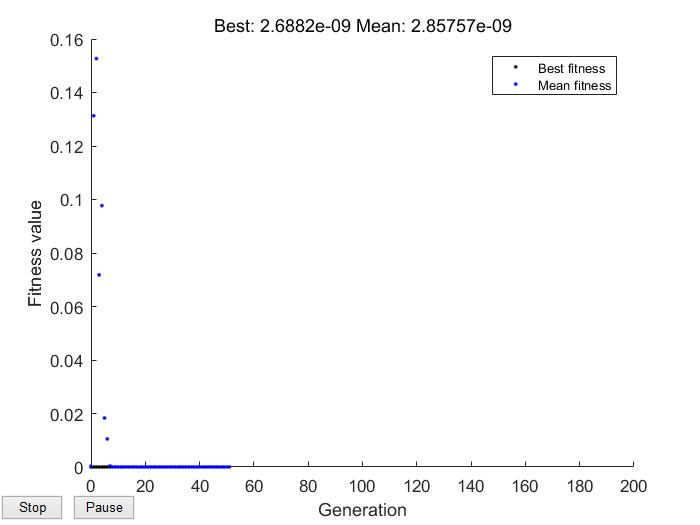
\includegraphics[width=\textwidth]{images/GA_taiyangyingzi_1.jpg}
                        \caption{}
                        \label{fig:太阳影子遗传算法迭代图}
                    \end{subfigure}
                    \begin{subfigure}[b]{0.4\textwidth}
                        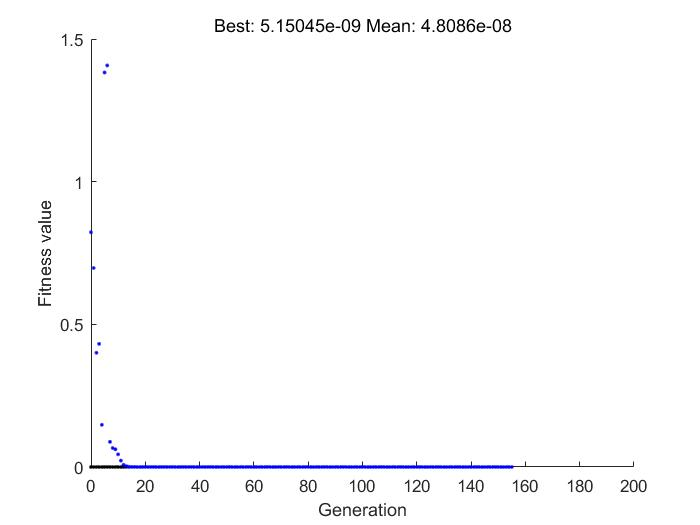
\includegraphics[width=\textwidth]{images/GA_taiyangyingzi_2.jpg}
                        \caption{}
                        \label{fig:不设置初始种群的遗传算法进化图}
                    \end{subfigure}
                    \caption{遗传算法迭代图}
                \end{figure}

    \subsection{问题三的分析与求解}
        \subsubsection{问题的分析}
            \par
            根据某固定直杆在水平地面上的太阳影子顶点坐标数据,建立数学模型确定直杆所处的地点和日期。将你们的模型分别应用于附件2和附件3的影子顶点坐标数据,给出\underline{若干个可能}的地点与日期。
            \par
            和第二问不同的是,这里不仅要求杆的地点$\varphi,\theta$,还要求拍摄日期$n$。这里我们仍然可以使用第二问中的三个优化模型,不过这里会增加一个新的优化变量(日期$n$),并且这个参数是整数型变量,与经纬度的实值型变量不同。对于这一点,我们要重新讨论。
            \par
            如果采用搜索法求解,只需要对日期也进行搜索即可:得到365天的最优解及最优值,然后在得到的365个最优值中选取最优解(这种方法好像有些问题)。如果采用牛顿法,不应将日期$n$作为实值型变量,可将优化算法与搜索法结合,对日期进行枚举,对每一天采用优化算法求解。
        \subsubsection{模型的建立与求解}
            \par
            单纯采用太阳影子长度进行求解的效率不是很高,因此,我们需要更多的影子信息。注意到,根据附件中的坐标信息$x_i,y_i$,我们还可以求出影子的角度。但是附件数据并未说明坐标轴是如何选取的,这使得问题变得困难。像未知高度$h$一样,我们可以将方位角进行相除,得到方位角变化情况。仅考虑影子角度的相对变化(即影子角度的改变量),这会方便我们建立坐标系$xOy$,因为不需要过多关注$x$和$y$轴的真实方向,建立影子角度变化模拟图如图(\ref{fig:太阳影子角度变化模拟图})
			\begin{figure}[H]
			\centering
			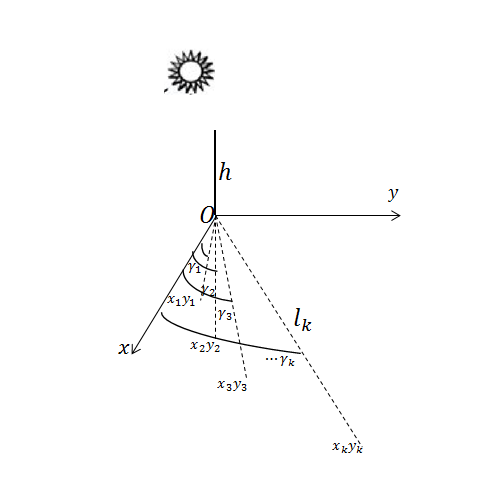
\includegraphics[height=5.5cm]{images/Sun_shadow_angle_change.jpg}
			\caption{太阳影子角度变化模拟图}
			\label{fig:太阳影子角度变化模拟图}
			\end{figure}
            图(\ref{fig:太阳影子角度变化模拟图})中的$h$代表杆高,$O$为杆高地点,$l_k$为第$k$个影长观测值,$(x_i, y_i )$表示第$i(i=1,2,\dots,k)$个影长在$xOy$坐标系的顶点坐标,$\hat{\gamma}_i$为第$i$个影子角度的大小(影角)的观测/估计,其计算公式为
            \begin{align*}
            \hat{\gamma}_i = \arctan\frac{y_i}{x_i}
            \end{align*}
            \par
            上面给出了影角的观测值求解方法,下面,我们给出影角的理论公式。考虑图(\ref{fig:太阳照射点的投影向量})的情况,杆$h$的影长公式为
            \begin{align*}
            l = \frac{h}{\tan\rho}
            \end{align*}
            太阳光在地面上的投影向量为
            \begin{align*}
            \vec{l} = \vec{m} - (\vec{m}\cdot \vec{n})\vec{n}
            \end{align*}
            其长度平方为
            \begin{align*}
            |\vec{l}|^2 = |\vec{m} - (\vec{m}\cdot \vec{n})\vec{n}|^2 = |\vec{m}|^2 - |\vec{m}\cdot\vec{n}|^2 = 1-\sin^2\rho = \cos^2\rho
            \end{align*}
            $O$点的正北方向为$O$指向北极的方向在$O$点出切平面的单位投影向量,也就是$z$轴正想在切平面上的单位投影向量,即
            \begin{align*}
            \mathbf{N} = \frac{\vec{z} - (\vec{z}\cdot\vec{n})\vec{n}}{|\vec{z} - (\vec{z}\cdot\vec{n})\vec{n}|}
            \end{align*}
            由于
            \begin{align*}
            \vec{z} - (\vec{z}\cdot\vec{n})\vec{n} = (-\sin\varphi\cos\varphi\cos w,-\sin\varphi\cos\varphi\sin w,\cos^2\varphi)
            \end{align*}
            其长度平方为
            \begin{align*}
            |\vec{z}|^2 - |\vec{z}\cdot\vec{n}|^2 = 1-\sin^2\varphi = \cos^2\varphi
            \end{align*}
            因此
            \begin{align*}
            \mathbf{N} = (-\cos w\sin\varphi,-\sin w\sin\varphi,\cos\varphi)
            \end{align*}
            于是,正北方向$\mathbf{N}$旋转至太阳影子方向的角度(影角)$\gamma$满足
            \begin{align*}
            \mathbf{N}\cdot\vec{l} = \cos\rho\cos \gamma = \cos\delta\cos w\sin\varphi - \sin\delta\cos \varphi
            \end{align*}
            即
            \begin{align*}
            \cos \gamma = \frac{\cos\delta\cos w\sin\varphi - \sin\delta\cos \varphi}{\cos\rho}
            \end{align*}
            注意,这里定义的影角与地学中定义的太阳方位角互为补角:余弦相差一个负号,正弦相同。结合$\sin\delta$的计算公式,上式可以写为
            \begin{align*}
            \cos\gamma = \frac{\sin\rho\sin\varphi - \sin\delta}{\cos\rho\cos\varphi}
            \end{align*}
            \par
            另一方面,地球的正东方向为
            \begin{align*}
            \mathbf{E} = \mathbf{N}\times \vec{n}=(-\sin w,\cos w,0)
            \end{align*}
            因而
            \begin{align*}
            \mathbf{N}\cdot \vec{l} = |\mathbf{E}||\vec{l}|\cos (\frac{\pi}{2} - \gamma) = \cos\rho\sin \gamma = \mathbf{E}\cdot\vec{m} = \sin w\cos\delta
            \end{align*}
            即
            \begin{align*}
            \sin \gamma = \frac{\sin w\cos\delta}{\cos\rho}
            \end{align*}
            同时给出$\sin \gamma$和$\cos\gamma$是为了避免出现影角$\gamma$多解的情况。
            \par
            和问题二中的处理方法相似,考虑影角相对变化以抵消$x$轴方向,建立影角的最小二乘目标
            \begin{align*}
            J({n,\varphi,\theta}) = \sum_{i=1}^k [(\gamma_{i+1}-\gamma_i)- (\hat{\gamma}_{i-1}-\hat{\gamma}_i)]^2
            \end{align*}
            将上述目标和影长的最小二乘目标相结合,设置目标权重$c$,有
            \begin{align*}
            & \min_{n,\varphi,\theta} \ J({n,\varphi,\theta}) = \sum_{i=1}^k\left\{ \left( \frac{l_{i+1}}{l_i} - \frac{\hat{l}_{i+1}}{\hat{l}_i} \right) ^2+c[(\gamma_{i+1}-\gamma_i)- (\hat{\gamma}_{i-1}-\hat{\gamma}_i)]^2 \right\}\\
            & s.t.\left\{
            \begin{aligned}
            & -90^\circ<\varphi<90^\circ\\
            & \rho_i>0\\
            & i=1,2,\dots,k
            \end{aligned}
            \right.
            \end{align*}

        \subsubsection{程序}
        \subsubsection{结果}

% \bibliography{taiyangyingzi}%bib文件名称
% \end{document}
